\documentclass{article} 
\usepackage{graphicx} % Required for inserting images
\usepackage[a4paper, left=2cm, right=2cm, top=2cm, bottom=2cm]{geometry}
\usepackage{tikz}
\usepackage{amsmath, amssymb}
\usepackage{fancyhdr}
\pagestyle{fancy}
\fancyhf{}

\fancyhead[L]{Student : Kuldeep(23684)}  % Left side
\fancyhead[C]{AI-ML (UMC203)}               % Centered
\fancyhead[R]{Instructor : Chiranjib Bhattacharyya}           % Right side

\begin{document}
    \thispagestyle{empty}
    \begin{center}
        \huge{\textbf{Artificial Intelligence and Machine Learning}} \\ 
        \vspace{1cm}
        \huge{\textbf{Assignment 01}} \\ 
        \vspace{2cm}
        \huge{\textbf{Instructor : Prof. Chiranjib Bhattacharyya}} \\
        \vspace{0.5cm}
        \huge{\textbf{Student : Kuldeep Jatav}} \\
        \vspace{0.5cm}
        \huge{\textbf{SR Number: 23684}} \\ 
        \vspace{3cm}

        
\includegraphics[width=0.5\textwidth]{IIScLogo.jpg}
    \end{center}
    
    \newpage
\noindent    \textbf{Solution 1 : Fisher's Linear Discriminant}

\begin{itemize}
    \item \textbf{Estimation (1.1):} Given RGB image dataset i build a four class classifier using Fisher's Linear Discriminant.
    
    From oracle using my SR Number i got a tuple with 5 elements as follows
    \begin{itemize}
        \item Tuple with two elements representing attributes of the dataset \textit{('Mouth\_Slightly\_Open', 'Smiling')}
        \item Train Image dataset $(dim = 20000 \times 3 \times 32 \times 32)$
        \item Train Label dataset $(dim = 20000 \times 1)$
        \item Test Image dataset  $(dim = 1000 \times 3 \times 32 \times 32)$
        \item Test Label dataset $(dim = 1000 \times 1)$
    \end{itemize}
    After this i caclulated $L_2$ norm of mean and $Frobenius$ $Norm$ of covarience matrices for each class taking subsamples of sizes $n=50,100,500,1000,2000,4000$ also the plot of $L_2$ norm of mean and $Frobenius$ $Norm$ of covarience matrices for each class is shown below. 
    
    if the mean vector is $x=\begin{bmatrix}
        x_1 , x_2 \dots x_d
    \end{bmatrix}$ and the covarience matrix is $C \in \mathbb{R}^d$ with $C_{ij}$ being element corrosponding to $i^{th}$ row and $j^{th}$ column of covarience matrix then 

    \[
    L_2 \hspace{3pt} Norm \hspace{3pt}= \sqrt{\sum_{i=1}^{d} (x_i)^2} \hspace{1cm} Frobenius \hspace{3pt} Norm \hspace{3pt} = \sqrt{\sum_{i=1}^{d} \sum_{j=1}^{d} (C_{ij})^2}
    \]
    \begin{figure}[h]
        \centering
        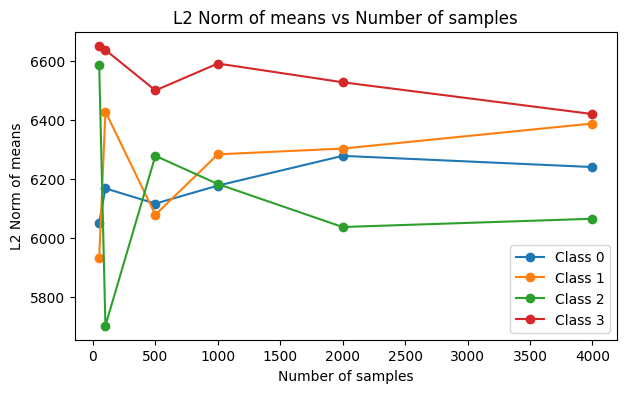
\includegraphics[width=0.69\textwidth]{L2_Norm.png} % Change filename if needed
        % \caption{L2 Norm of Mean}
        \label{fig:L2_Norm}
    \end{figure}

    \begin{figure}[h]
        \centering
        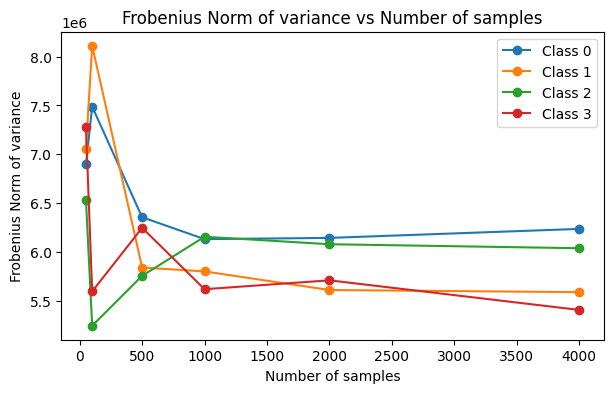
\includegraphics[width=0.69\textwidth]{Frob_Norm.png} % Change filename if needed
        % \caption{L2 Norm of Mean}
        \label{fig:Frob_Norm}
    \end{figure}

    \item \textbf{FLD Implementation(1.2.a) :} For each of 4 class with number of subsamples $n = 2500, 3500, 4000, 4500, 5000$ 
    \item \textbf{Theory :} Fisher's Linear Discriminant is a dimensionality reduction technique that finds the linear combination of features that maximizes the separation between multiple classes. It does this by maximizing the between-class variance while minimizing the within-class variance. 
    
    Suppose we have $C$ classes and $d$ features \& the within-class scatter matrix $S_W$ is defined as follows
    \[ S_W = \sum_{i=1}^{C} S_i \]
    where $S_i$ is the scatter matrix for $i^{th}$ class
    \[ S_i = \sum_{x \in X_i} (x - m_i)(x - m_i)^T \]
    where $X_i$ is the set of samples for $i^{th}$ class and $m_i$ is the mean vector for $i^{th}$ class.

    and between-class scatter matrix $S_B$ is defined as follows
    \[ S_B = \sum_{i=1}^{C} N_i (m_i - m)(m_i - m)^T \]
    where $m$ is the overall mean vector and $N_i$ is the number of samples in $i^{th}$ class.

    The Fisher's Linear Discriminant is defined as the vector $w$ that maximizes the ratio of between-class scatter to within-class scatter.
    \[ w = argmax  \left( \frac{w^T S_B w}{w^T S_W w} \right) \]

    Objective function value of fisher's linear discriminant is defined as follows
    \[ J(w) = \frac{|w^T S_B w|}{|w^T S_W w|} \hspace{7pt} \text{where $|X| $ represents determinant of $X$} \]

    \item \textbf{Box Plot} for the multiclass objective value of the Fisher's Linear Discriminant for different $n$.
        \begin{figure}[h]
            \centering
            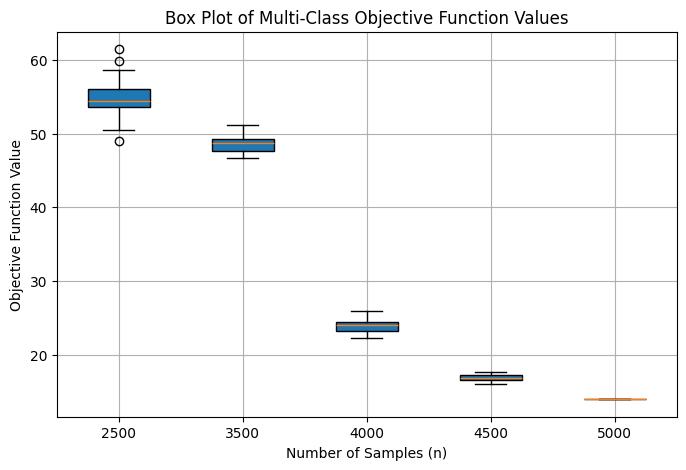
\includegraphics[width=0.69\textwidth]{BoxPlot.png} 
            \label{fig:box_plot}
        \end{figure}
        
\newpage
        
    
     \item \textbf{Projections} of 5000 points from training dataset in $3D$.
        \begin{figure}[h]
            \centering
            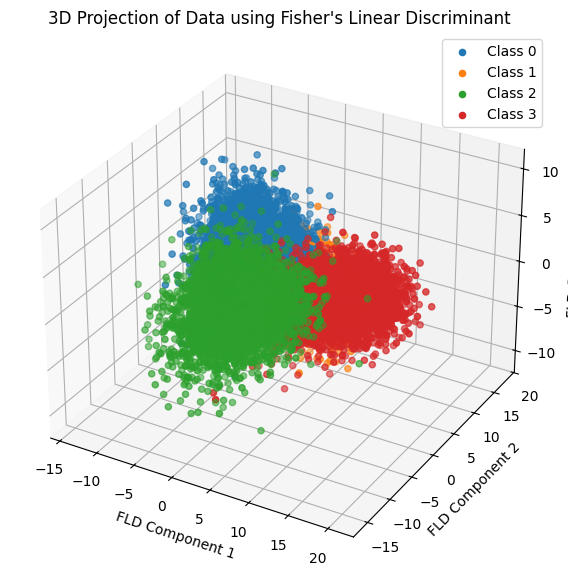
\includegraphics[width=0.6\textwidth]{Projection.png}
            \label{fig:Projection}
        \end{figure}
        % \item \textbf{Threshold Report} 
    \item \textbf{Threshold Report} for the given dataset is as follows
    \begin{figure}[h]
        \centering
        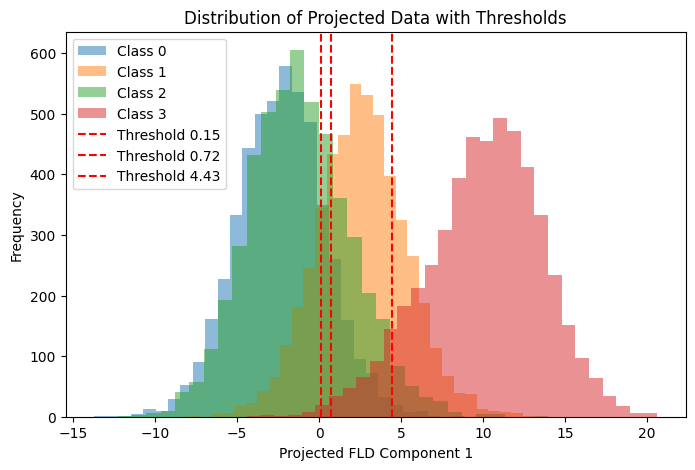
\includegraphics[width=0.6\textwidth]{threshold.png} % Change filename if needed
        % \caption{L2 Norm of Mean}
        \label{fig:Threshold}
    \end{figure}
    
    \item \textbf{Accuracy on Test Data(1.2.b) :} 74.20\% (Please refer Code)
\end{itemize}


\noindent \textbf{Solution 2 : Bayes Classification}  

\begin{itemize}
    \item    \textbf{Theory : } Bayes Classifier is a probabilistic model that makes a decision based on the probability of an event. It is based on Bayes' theorem.
        \[ P(Y|X) = \frac{P(X|Y)P(Y)}{P(X)} \]

        \[\eta(x) = \frac{P(Y=1 \mid X=x) \times P(Y=1)}{P(X=x)} \]
        \[1-\eta(x) = \frac{P(Y=0 \mid X=x) \times P(Y=0)}{P(X=x)} \]
        and hence we classify $x$ as 
        \[
    \text{Classifier} = \begin{cases}
            1 \hspace{37pt} \text{ if } \eta(x) \geq \frac{1}{2} + \epsilon \\
            0 \hspace{37pt} \text{ if } \eta(x) \leq \frac{1}{2} - \epsilon \\
            \text{Reject} \hspace{14pt} \text{ otherwise}
        \end{cases}
        \]
        Equivalently we can say classify $x$ as 1 if
        \[
            \frac{\eta(x)}{1-\eta(x)} \geq \frac{\frac{1}{2}+\epsilon}{\frac{1}{2}-\epsilon} \hspace{10pt} \text{or} \hspace{10pt} log \left( \frac{\eta(x)}{1-\eta(x)} \right) \leq log \left( \frac{\frac{1}{2}+\epsilon}{\frac{1}{2}-\epsilon} \right)
        \]
        and classify $x$ as 0 if
        \[
            \frac{\eta(x)}{1-\eta(x)} \leq \frac{\frac{1}{2}-\epsilon}{\frac{1}{2}+\epsilon} \hspace{10pt} \text{or} \hspace{10pt} log \left( \frac{\eta(x)}{1-\eta(x)} \right) \geq log \left( \frac{\frac{1}{2}-\epsilon}{\frac{1}{2}+\epsilon} \right)
        \]
        Rejce the sample if none of the above conditions are satisfied \& $log \left( \frac{\eta(x)}{1-\eta(x)} \right)$ can be calculate as follows

        \[ log \left( \frac{\eta(x)}{1-\eta(x)} \right) = log \left( \frac{P(Y=1 \mid X=x) \times P(Y=1)}{P(Y=0 \mid X=x) \times P(Y=0)} \right) \]

        \[= -\frac{1}{2} (x - \mu_1)^T C_1^{-1} (x - \mu_1) 
    + \frac{1}{2} (x - \mu_2)^T C_2^{-1} (x - \mu_2) 
    - \frac{1}{2} log |C_1| + \frac{1}{2} log |C_2|\]
    \item \textbf{Modified Bayes Classifier(2.1 , 2.2) :} From oracle for question 2 i got two element tuples as follows
    \begin{itemize}
        \item Training dataset $(dim = 4800 \times 785)$
        \item Test dataset $(dim = 800 \times 785)$
    \end{itemize}
    where the first column is labels corrosponding to each of 784 features.

    we are aksed to implement a modified bayes classifier as follows
    \[
    h_{\epsilon}(x) = \begin{cases}
        1 \hspace{37pt} \text{ if } \eta(x) \geq \frac{1}{2} + \epsilon \\
        0 \hspace{37pt} \text{ if } \eta(x) \leq \frac{1}{2} - \epsilon \\
        \text{Reject} \hspace{14pt} \text{ otherwise}
    \end{cases}
    \]
    where $\eta(x) = P(Y=1|X=x)$ and $\epsilon \in (0,0.5) $ is a threshold parameter. 

    for each $\epsilon \in \{0.01,0.1,0.25,0.4\}$ we have to find the following on the dataset
    \begin{itemize}
        \item Misclassification Loss among the non-rejected samples
        \item Number of rejected samples  
    \end{itemize}

    In next part we have to do the same for but with different split of training (60-40 , 80-20 , 90-10 , 99-1).

    

    I have implemented both simulteneously and got the following results.
    \begin{figure}[h]
        \centering
        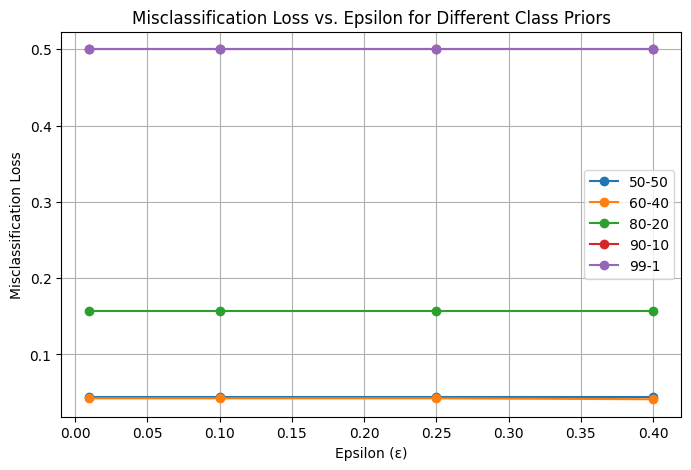
\includegraphics[width=0.69\textwidth]{Misclassification.png} % Change filename if needed
        % \caption{L2 Norm of Mean}
        \label{fig:Bayes}
    \end{figure}

    % Following tables shows the summary of the results from plot.
    \begin{itemize}
        \item \textbf{Misclassification Loss}
        \begin{table}[h]
            \centering
            \begin{tabular}{|c|c|c|c|c|}
                \hline
                {split/$\mathbb{\epsilon}$} & \textbf{0.01} & \textbf{0.1} & \textbf{0.25} & \textbf{0.4} \\
                \hline
                50-50 & 0.04375 & 0.04375 & 0.04375 & 0.04375 \\ \hline
                60-40 & 0.0425 & 0.0425 & 0.0425 & 0.04130162703379224 \\ \hline
                80-20 & 0.1575 & 0.1575 & 0.1575 & 0.1575 \\ \hline
                90-10 & 0.5 & 0.5 & 0.5 & 0.5 \\ \hline
                99-1 & 0.5 & 0.5 & 0.5 & 0.5 \\ \hline
            \end{tabular}
        \end{table}
% \newpage
        \item \textbf{Number of Rejected Samples}
        \begin{table}[h]
            \centering
            \begin{tabular}{|c|c|c|c|c|}
                \hline
                {split/$\mathbb{\epsilon}$} & \textbf{0.01} & \textbf{0.1} & \textbf{0.25} & \textbf{0.4} \\ \hline
                50-50 & 0 & 0 & 0 & 0 \\ \hline 
                60-40 & 0 & 0 & 0 & 0 \\ \hline
                80-20 & 0 & 0 & 0 & 0 \\ \hline
                90-10 & 0 & 0 & 0 & 0 \\ \hline
                99-1 & 0 & 0 & 0 & 0 \\ \hline
            \end{tabular}
        \end{table}
    \end{itemize}


    \item \textbf{K-Fold Cross Validation (2.3.a , 2.3.b) :} In this part we have to implement K-Fold Cross Validation for the given dataset and we are allowed to use the inbuilt function \textit{K-Fold} from \textit{sklearn.model\_selection}.
    
    You can refer the code for the implementation of K-Fold Cross Validation in the code file. I got the following results after implementing K-Fold Cross Validation.
    \begin{itemize}
        \item Recall : 0.9300339683788492
        \item Precision : 0.9510064802802078
        \item F1 Score : 0.9403905714487368
        \item Accuracy : 0.9410416666666667
        \item Confusion Matrix
        \[CM = \begin{bmatrix}
            TN & FP \\
            FN & TP
        \end{bmatrix} = \begin{bmatrix}
            451 & 25 \\
            33 & 451
        \end{bmatrix}\]
        \item Misclassification Loss : 0.0589583333333332
        \item Number of Rejected Samples : 0
    \end{itemize}

\end{itemize}



% \newpage

\noindent    \textbf{Solution 3 : Decision Trees}
\begin{itemize}
    \item \textbf{Visualization (3.1) :}  You can zoom the following decision tree and see the details.
    
    \begin{figure}[h]
        \centering
        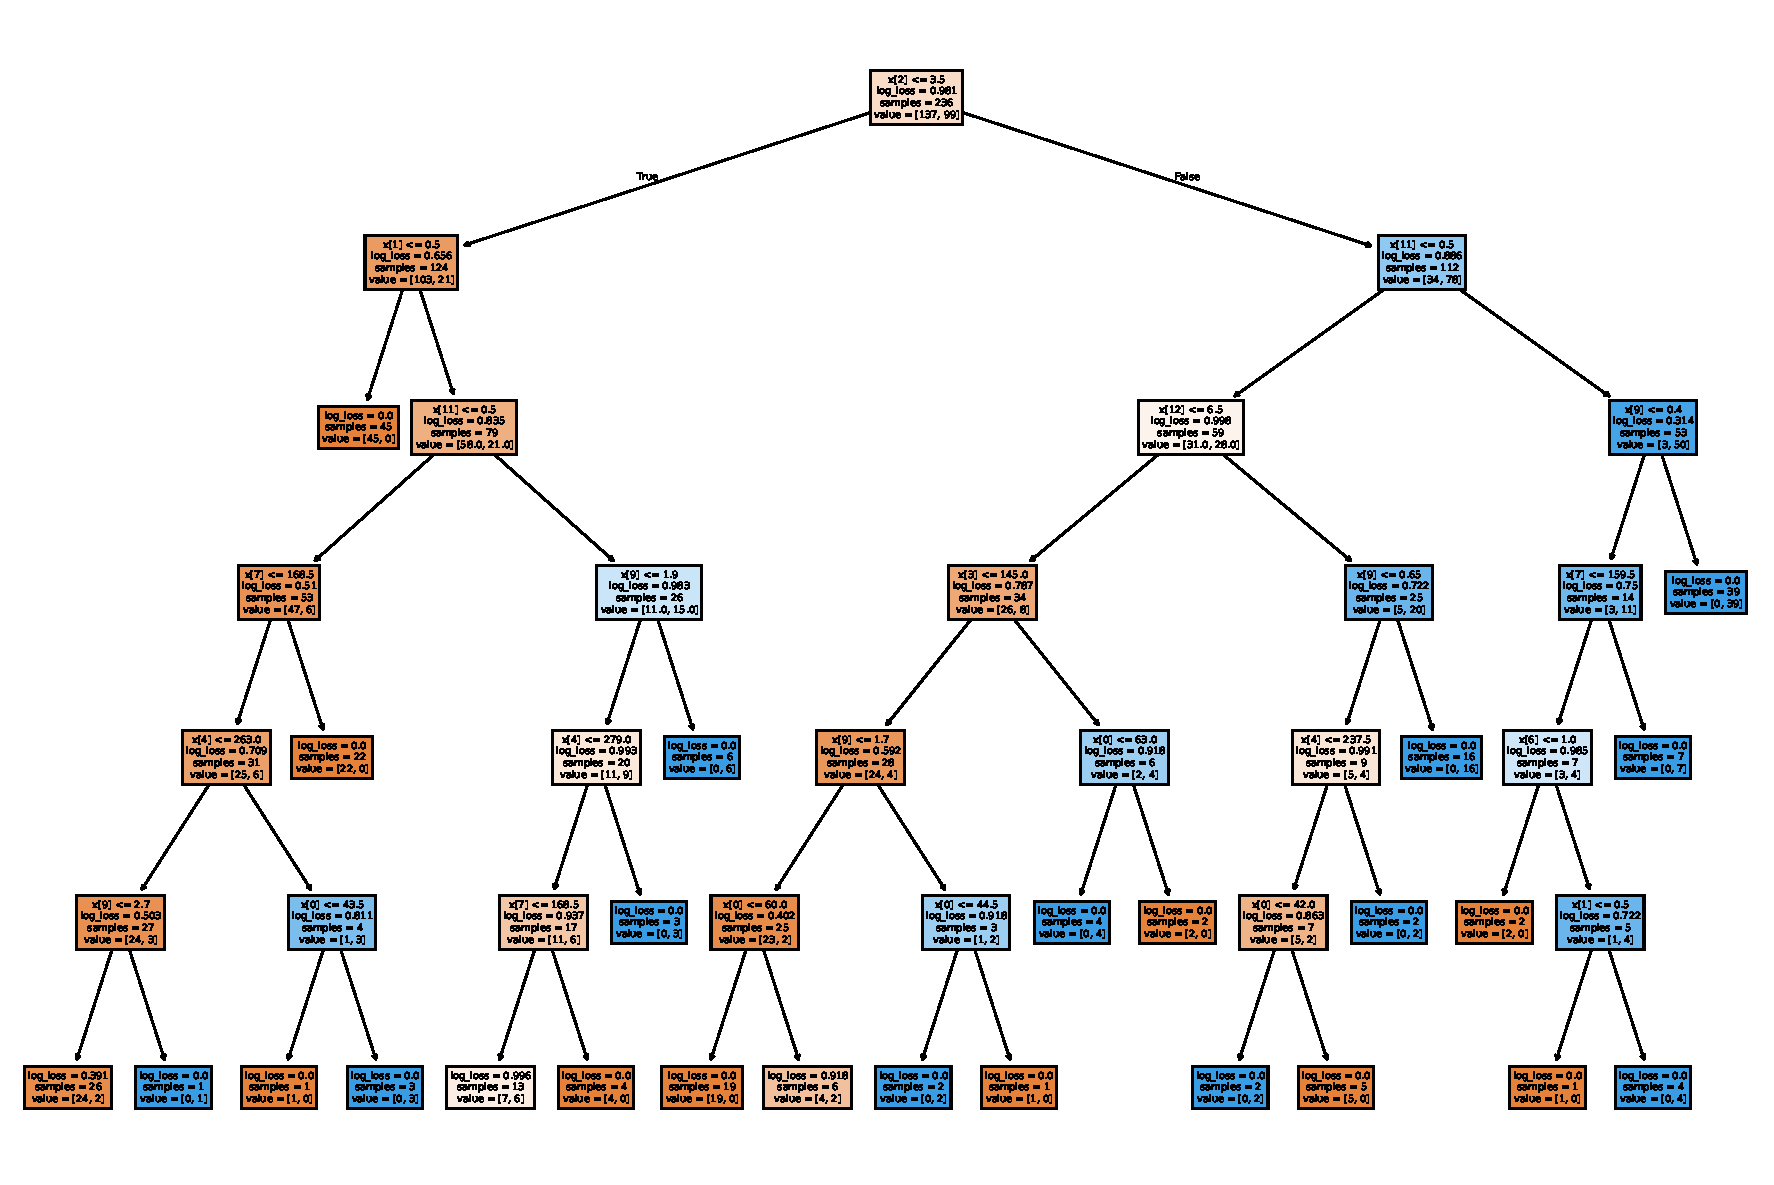
\includegraphics[width=\textwidth]{decision_tree.pdf} % Change filename if needed
        % \caption{Decision Tree Visualization}
        \label{fig:decision_tree}
    \end{figure}

    \item \textbf{Report (3.2) :} from oracle for question 3 i got (\textit{log\_loss, best, 6}) as hyperparameters for Decision Tree Classifier  where \textit{log\_loss} is the criterion, \textit{best} is the splitter and \textit{6} is the max\_depth in decision tree.
    
    Suppose $TP,TN,FP,FN$ represent True Positive, True Negative, False Positive and False  Negative \newline respectively then the following formulas are used to calculate the performance of the model.
    \[\text{Precision = } \frac{TP}{TP+FP} \]
    \[\text{Accuracy = } \frac{TP+FN}{TP+FP+TN+FN} \]
    \[\text{Recall = } \frac{TP}{TP+FN} \]
    \[\text{F1 Score = } \frac{2*Precision * Recall}{Precision + Recall }\]
    
    after training the model with these hyperparameters i got the following results on test data. 
    \[TN = 17 \hspace{3pt},\hspace{3pt} FP = 5 \hspace{3pt},\hspace{3pt} FN = 9 \hspace{3pt} , \hspace{3pt} TP = 29 \]
    \begin{itemize}
        \item Precision : 0.8484848484848485 
        \item Accuracy : 0.75
        \item Recall : 0.7368421052631579
        \item F1 Score : 0.7887323943661972
        \item Training Data Accuracy
        \begin{itemize}
            \item Before Pruning : 1.000000000000000
            \item After Pruning : 0.9576271186440678
        \end{itemize}
        \item Confusion Matrix : Suppose $C$ denotes the confusion matrix then
        \[C = \begin{bmatrix}
            TN & FP \\
            FN & TP
        \end{bmatrix} = \begin{bmatrix}
            17 & 5 \\
            9 & 29
        \end{bmatrix}\]
    \end{itemize}

    \item \textbf{Best Feature (3.3) :} The best feature in a Decision Tree is the one that provides the most informative split, meaning it reduces impurity (Gini or Entropy or log\_loss) the most. we can deduce the best feature using feature importance scores and tree structure analysis.
    
    Feature 2 is the root node in the decision tree which means the decision tree chose it as the first splitting feature because it provides the most information gain hence the most important feature is \textbf{Feature 2}.

    Using Inbuilt Python Function \boxed{\textit{feature\_importances\_}} I got the following order of importance of features.

    \[ 2 > 11 > 9 > 0 > 1 > 7 > 4 > 12 > 3 > 6 > 10 > 8\]

    \textbf{Note : }It is 0 Index order! (we can add 1 to each index to get the actual feature number)
\end{itemize}

\vspace{1cm}

\begin{center}
    \text{\Huge{\textbf{Thank You!}}}
\end{center}

\end{document}